\chapter{General Context}
\minitoc % Generates a mini table of contents for this chapter
\section*{Introduction}
This chapter outlines the project's general framework, introduces the hosting organization, and details the core challenges identified. In addition, it describes the proposed technical solution, the development environment, the chosen technology stack, and the Agile methodology used. Finally, it introduces the Unified Modeling Language (UML) for system design and presents the global MVC architecture of the ERP back-end system.

\section{General Frame of the Project}
The digital transformation of modern enterprises necessitates powerful, integrated tools that provide managers with comprehensive control over daily operations. Enterprise Resource Planning (ERP) systems are central to this transformation, consolidating disparate functions—such as finance, human resources, sales, and inventory—into a single, unified platform to streamline processes and improve data coherence.

This internship project focused on the design and development of the \textbf{backend infrastructure for a customized ERP system}, specifically tailored to the needs of small and medium-sized enterprises (SMEs). As the \textbf{backend developer}, my core responsibilities encompassed:
\begin{itemize}
    \item Designing and developing a complete set of \textbf{RESTful APIs} using the Laravel framework.
    \item Implementing a secure \textbf{JWT (JSON Web Token)} authentication and authorization system.
    \item Architecting, designing, and managing the relational database using \textbf{MySQL}.
    \item Rigorously testing all API endpoints for reliability and performance using \textbf{Postman}.
    \item Adhering to the \textbf{Agile Scrum methodology}, utilizing \textbf{ClickUp} for task management, sprint planning, and progress tracking.
\end{itemize}

\section{Hosting Organization}
\subsection{General Overview}
The internship was carried out at \textbf{Anter Lab}, a Tunisian company founded by \textit{Mohamed Amine Jalel} and \textit{Aymen Sahraoui}. Anter Lab is an innovative software development company that specializes in the creation of \textbf{ERP systems, HR platforms, and digital transformation solutions}. The company’s mission is to \textbf{empower SMEs, startups, and associations by providing modern tools to streamline their processes and optimize resource management}.

\subsection{Vision and Mission}
Anter Lab’s vision is to become a leader in digital solutions that simplify enterprise management in Tunisia and abroad.  
Its mission revolves around:
\begin{itemize}
    \item Providing \textbf{custom-built ERP and HR solutions} that adapt to the specific needs of each organization.
    \item Offering \textbf{digital tools} that facilitate collaboration, communication, and data-driven decision-making.
    \item Supporting companies and associations in their \textbf{digital transformation journey}.
\end{itemize}

\subsection{Areas of Expertise}
The company’s main expertise areas are:
\begin{itemize}
    \item \textbf{Enterprise Resource Planning (ERP):} Custom ERP solutions to handle finance, HRM, projects, and operations.
    \item \textbf{Human Resources Platforms (HRM):} Tools for managing members, performance evaluation, and workflow automation.
    \item \textbf{Custom Web Applications:} Full-stack applications adapted to client requirements.
    \item \textbf{Consulting and Training:} Technical support, training sessions, and consultancy to ensure adoption and efficiency.
\end{itemize}

\subsection{Clients and Partnerships}
Anter Lab collaborates with:
\begin{itemize}
    \item \textbf{Associations and NGOs}, supporting digital transformation in community projects.
    \item \textbf{Startups}, helping them scale operations with customized platforms.
    \item \textbf{SMEs}, providing management tools for HR, finance, and daily operations.
\end{itemize}

\subsection{Organization and Structure}
The structure of Anter Lab is built around an agile and collaborative environment, with the following main departments:
\begin{itemize}
    \item \textbf{Management:} Responsible for company strategy and business decisions.
    \item \textbf{Technical Development:} Teams of backend, frontend, and full-stack developers.
    \item \textbf{Design and UX:} Specialists in UI/UX to ensure product usability.
    \item \textbf{Consulting and Support:} Assisting clients through training, maintenance, and technical guidance.
\end{itemize}

\begin{figure}[H]
    \centering
    \begin{tikzpicture}[
        node distance=1.8cm and 2.8cm,
        box/.style={
            draw, 
            rectangle, 
            rounded corners=4pt,
            minimum width=3.2cm, 
            minimum height=0.9cm,
            align=center,
            text width=2.9cm,
            font=\footnotesize,
            fill=blue!10
        },
        root/.style={
            box,
            fill=blue!25,
            font=\bfseries,
            minimum width=4cm,
            text width=3.5cm
        },
        dept/.style={
            box,
            fill=blue!20,
            font=\bfseries
        },
        person/.style={
            font=\scriptsize,
            align=center,
            text width=2.5cm
        },
        arrow/.style={
            ->,
            thick,
            shorten >=3pt,
            shorten <=3pt
        }
    ]

   % Root node - centered at top
    \node[root] (ceo) {General Management};
    % Departments - properly spaced in a row
    \node[dept, below=2.5cm of ceo, xshift=-5cm] (dev) {Development Department};
    \node[dept, below=2.5cm of ceo] (prod) {Product \& Consulting Department};
    \node[dept, below=2.5cm of ceo, xshift=5cm] (support) {Support \& Training Department};
    
    % Connect CEO to departments with clean lines
    \draw[arrow] (ceo.south) -- ++(0,-0.7) -| (dev.north);
    \draw[arrow] (ceo.south) -- (prod.north);
    \draw[arrow] (ceo.south) -- ++(0,-0.7) -| (support.north);
    
    % Development department teams - arranged vertically
    \node[box, below=1.5cm of dev] (backend) {Backend Team \\ (Java, PHP, Python)};
    \node[box, below=1.5cm of backend] (frontend) {Frontend Team \\ (JavaScript, modern frameworks)};
    \node[box, below=1.5cm of frontend] (data) {Data \& AI Team \\ (Python, Data Analysis, Cybersecurity)};
    
    % Connect development to its teams
    \draw[arrow] (dev.south) -- (backend.north);
    \draw[arrow] (backend.south) -- (frontend.north);
    \draw[arrow] (frontend.south) -- (data.north);
    
    % Product department teams - arranged vertically
    \node[box, below=1.5cm of prod] (rh) {HR Solutions Design};
    \node[box, below=1.5cm of rh] (erp) {ERP Solutions Design};
    \node[box, below=1.5cm of erp] (conseil) {Consulting and support \\ for associations};
    
    % Connect product to its teams
    \draw[arrow] (prod.south) -- (rh.north);
    \draw[arrow] (rh.south) -- (erp.north);
    \draw[arrow] (erp.south) -- (conseil.north);
    
    % Support department teams - arranged vertically
    \node[box, below=1.5cm of support] (tech) {Continuous technical support};
    \node[box, below=1.5cm of tech] (formation) {Training for using \\ HR/ERP solutions};
    \node[box, below=1.5cm of formation] (update) {System updates and \\ improvements};
    
    % Connect support to its teams
    \draw[arrow] (support.south) -- (tech.north);
    \draw[arrow] (tech.south) -- (formation.north);
    \draw[arrow] (formation.south) -- (update.north);
    
    % Clients node - positioned to the far right with clear separation
    \node[box, right=7cm of prod, fill=green!20] (clients) {Clients \\ (Associations \& Organizations)};
    \node[person, below=0.3cm of clients, text width=3.5cm] {Use ANTER LAB solutions to improve their internal management and performance};
    
    % Connect to clients - clean, direct arrows
    \draw[arrow] (prod.east) -- ++(1.5,0) |- ([yshift=2pt]clients.west);
    \draw[arrow] (conseil.east) -- ++(2.5,0) |- (clients.west);
    \draw[arrow] (support.east) -- ++(1.0,0) |- ([yshift=-2pt]clients.west);
    
    \end{tikzpicture}
    \caption{Organizational Structure of Anter Lab}
    \label{fig:org_chart}
\end{figure}

\section{Studying Critiques and Their Existence}
A critical analysis of existing market-leading ERP systems (e.g., Odoo, SAP, Microsoft Dynamics) was conducted prior to development. While powerful, these solutions present significant barriers for SMEs, including:
\begin{itemize}
    \item \textbf{Prohibitive Costs:} High licensing, implementation, and ongoing maintenance fees.
    \item \textbf{Implementation Complexity:} Steep learning curves and difficult, costly customization processes.
    \item \textbf{Scalability Challenges:} Solutions are often not cost-effectively adaptable to the evolving needs of a growing SME.
    \item \textbf{Operational Fragmentation:} Many businesses resort to multiple disjointed systems, leading to data silos and inefficient processes.
\end{itemize}

\section{Proposed Solution}
To address these challenges, we developed a modular and scalable backend for a custom ERP system. The proposed solution provides the following: 
\begin{itemize}
    \item A well-documented set of \textbf{RESTful APIs} to power core modules (HRM, POS, Finance, CRM).
    \item A robust and secure authentication mechanism using \textbf{JWT} to protect API endpoints.
    \item A normalized and efficient \textbf{MySQL} database schema ensuring data integrity and performance.
    \item A flexible architecture built with \textbf{Laravel}, allowing for easy future expansion and maintenance.
    \item A development process managed under \textbf{Scrum} to ensure timely delivery and adaptability to changing requirements.
\end{itemize}
\begin{figure}[H]
    \centering
    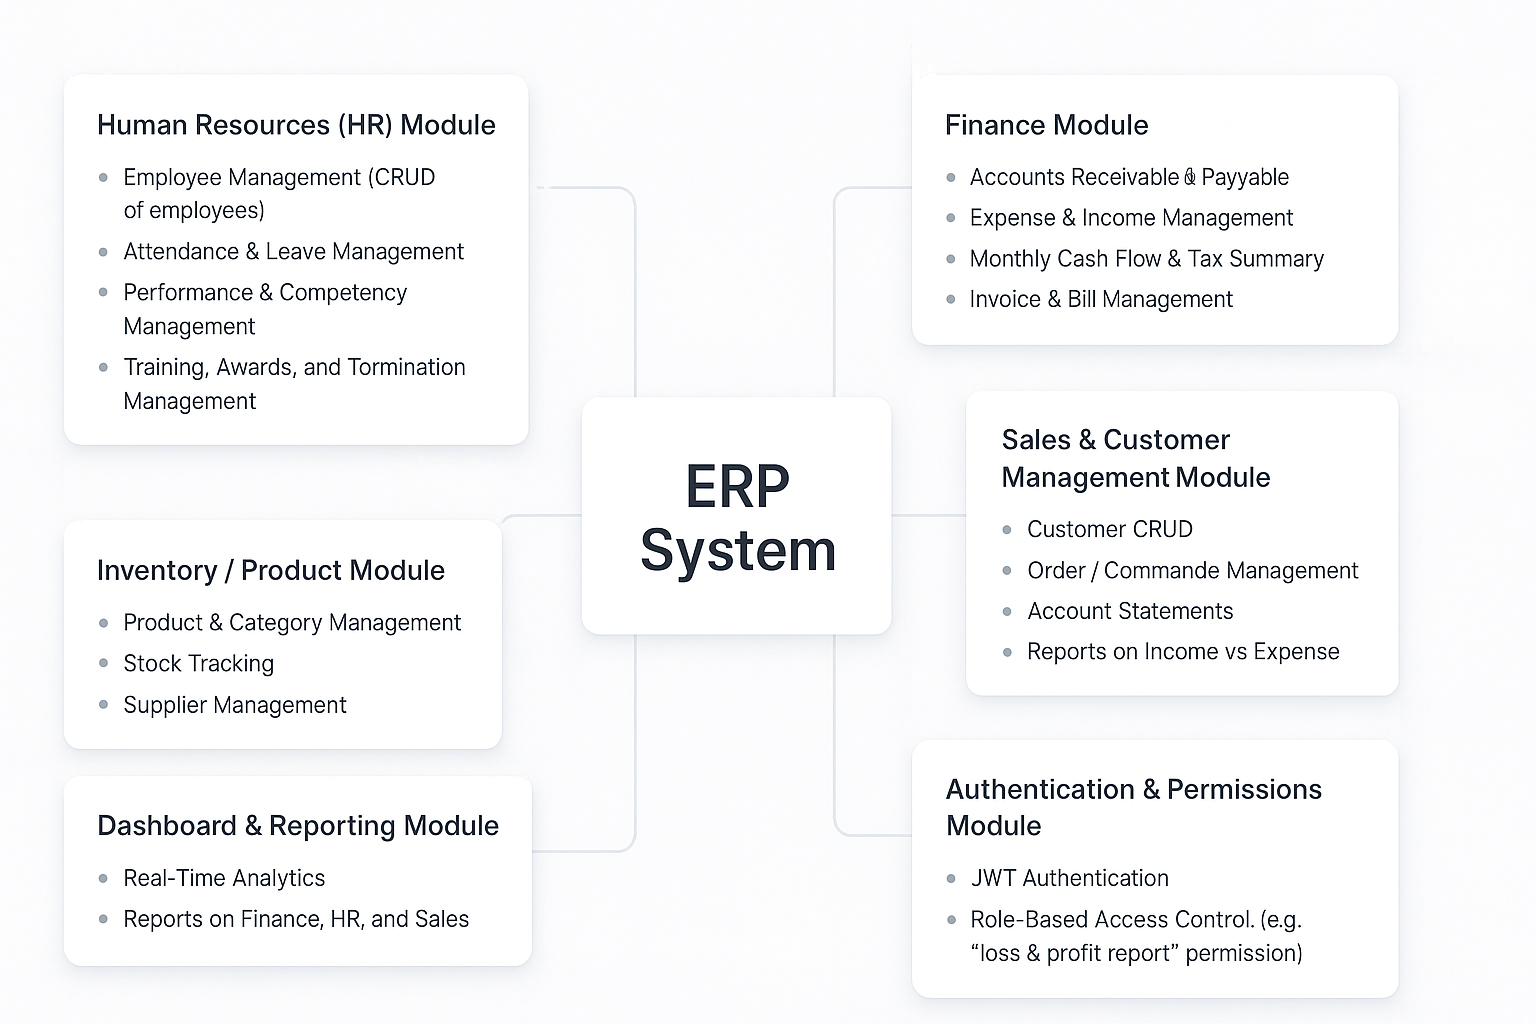
\includegraphics[width=0.7\textwidth]{chapters/chapter 1/figures/ERP_SYSTEM.png}
    \caption{High-Level Overview of the ERP System Modules}
    \label{fig:erp_modules}
\end{figure}

\section{Development Environment}
\subsection{Software Environment}
The development process was supported by a modern and efficient software toolset:
\begin{itemize}
    \item \textbf{Visual Studio Code:} Primary code editor for development.
    	\begin{figure}[H]
        \centering
        
\includegraphics[width=0.2\textwidth]{chapters/chapter 1/figures/vscode.png}
        \caption{Visual Studio Code}
        \label{fig:vscode}
    	\end{figure}
    \item \textbf{Postman:} Essential for API testing, debugging, and creating documentation for consumers.
    	\begin{figure}[H]
        \centering
        
\includegraphics[width=0.2\textwidth]{chapters/chapter 1/figures/postman.png}
        \caption{Postman API Platform}
        \label{fig:postman}
    	\end{figure}
    \item \textbf{Git \& GitLab:} Used for version control, code collaboration, and project synchronization, leveraging GitLab's integrated CI/CD and issue tracking features.
	\begin{figure}[H]
	\centering
	\begin{minipage}{0.35\textwidth}
		\centering
		
\includegraphics[width=0.6\linewidth]{chapters/chapter 1/figures/git.png}
		\subcaption{Git}
	\end{minipage}%
	\begin{minipage}{0.35\textwidth}
		\centering
		
\includegraphics[width=0.6\linewidth]{chapters/chapter 1/figures/gitLab.png}
		\subcaption{GitLab}
	\end{minipage}
	\caption{Version Control and Collaboration Tools}
	\label{fig:git_gitlab}
	\end{figure}
    \item \textbf{ClickUp:} Central hub for task management, sprint backlogs, and Agile workflow tracking.
    	\begin{figure}[H]
        \centering
        
\includegraphics[width=0.2\textwidth]{chapters/chapter 1/figures/clickUp.png}
        \caption{ClickUp Project Management}
        \label{fig:clickup}
    	\end{figure}
    \item \textbf{Overleaf / LaTeX:} Used for professional report writing, formatting, and collaborative documentation.
    	\begin{figure}[H]
        \centering
        
\includegraphics[width=0.2\textwidth]{chapters/chapter 1/figures/overleaf.jpg}
        \caption{Overleaf / LaTeX Environment}
        \label{fig:overleaf}
    	\end{figure}
   \item \textbf{PlantUML:} Used for creating UML diagrams such as use cases, class diagrams, sequence diagrams, and sequence diagrams.
    \begin{figure}[H]
        \centering
        
\includegraphics[width=0.2\textwidth]{chapters/chapter 1/figures/plantUml.png}
        \caption{PlantUML for UML Diagrams}
        \label{fig:plantuml}
    \end{figure}
\item \textbf{Draw.io:} Also employed for designing UML diagrams and system architecture visually.
    \begin{figure}[H]
        \centering
        
\includegraphics[width=0.2\textwidth]{chapters/chapter 1/figures/drawio.png}
        \caption{Draw.io for UML and Architecture Diagrams}
        \label{fig:drawio}
    \end{figure}
\item \textbf{Discord:} Platform for daily stand-ups, sprint reviews, and remote team communication.
    \begin{figure}[H]
        \centering
        
\includegraphics[width=0.2\textwidth]{chapters/chapter 1/figures/Discord-Logo.png}
        \caption{Discord Communication Platform}
        \label{fig:discord}
    \end{figure}
\end{itemize}

\subsection{Technological Choices}
The technology stack was selected to ensure performance, security, and long-term maintainability:
\begin{itemize}
    \item \textbf{Laravel:} A powerful PHP framework chosen for its elegant syntax, robust ecosystem, and built-in features that accelerate development (e.g., Eloquent ORM, Artisan).
    \item \textbf{JWT (JSON Web Tokens):} Selected for implementing stateless authentication, providing a scalable and secure way to manage user sessions across multiple devices.
    \item \textbf{MySQL:} A reliable, widely-used relational database management system ideal for handling the complex and structured data of an ERP.
    \item \textbf{REST API:} An architectural style chosen for its simplicity, statelessness, and compatibility with any front-end client (web, mobile, desktop).
    \item \textbf{LaTeX / Overleaf:} For professional, structured, and version-controlled report documentation.
    \item \textbf{PlantUML:} To programmatically generate UML diagrams ensuring maintainable and reproducible design documentation.
\end{itemize}
\begin{figure}[H]
    \centering
    % First row
    \begin{minipage}{0.45\textwidth}
        \centering
        
\includegraphics[width=\linewidth]{chapters/chapter 1/figures/laravel.png}
        \caption{Laravel}
        \label{fig:laravel}
    \end{minipage}%
    \hfill
    \begin{minipage}{0.45\textwidth}
        \centering
        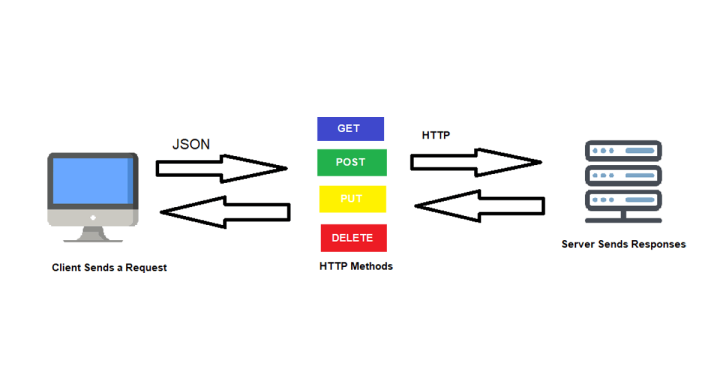
\includegraphics[width=\linewidth]{chapters/chapter 1/figures/rest-api.png}
        \caption{REST API}
        \label{fig:restapi}
    \end{minipage}

    \vspace{0.5cm} % vertical space between rows

    % Second row
    \begin{minipage}{0.45\textwidth}
        \centering
        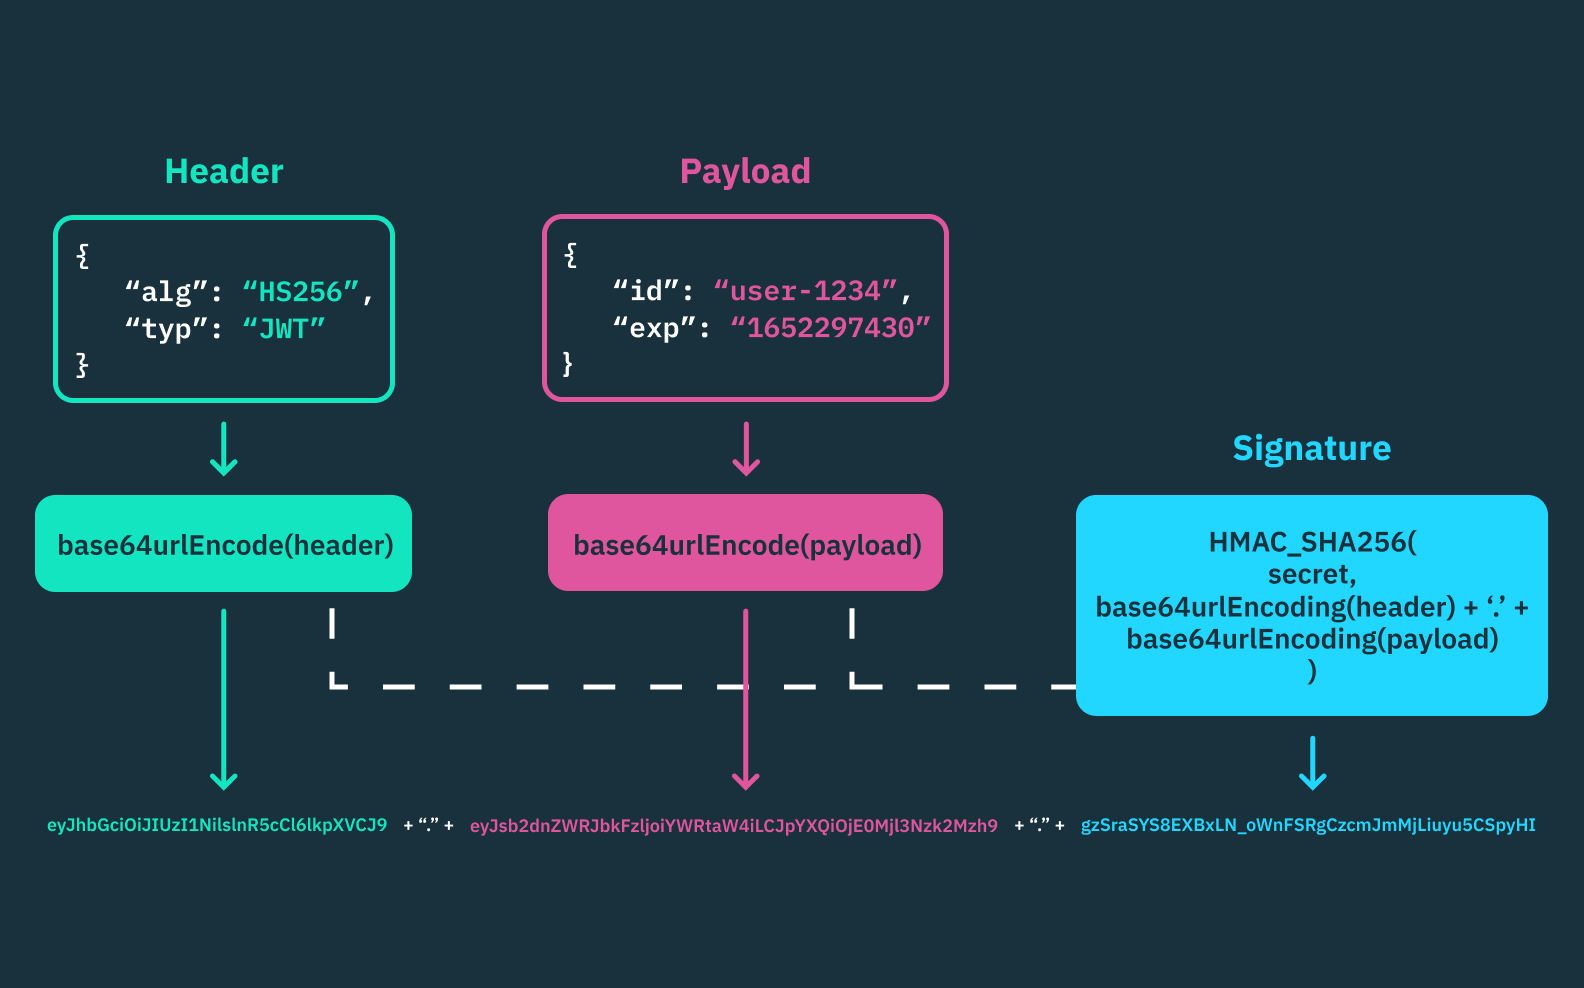
\includegraphics[width=\linewidth]{chapters/chapter 1/figures/jwt-struct.png}
        \caption{JWT}
        \label{fig:jwt}
    \end{minipage}%
    \hfill
    \begin{minipage}{0.45\textwidth}
        \centering
        
\includegraphics[width=\linewidth]{chapters/chapter 1/figures/mysql.png}
        \caption{MySQL}
        \label{fig:mysql}
    \end{minipage}
\end{figure}

\subsection{Choice of Methodology}
The project was executed using the \textbf{Agile methodology} with the \textbf{Scrum framework}. This iterative approach was crucial for managing evolving requirements, ensuring continuous delivery of value, and maintaining a high level of responsiveness to feedback.

\subsection{Presentation of the Scrum Methodology}
Scrum is an iterative Agile framework built on three pillars: \textbf{Transparency}, \textbf{Inspection}, and \textbf{Adaptation}.
\begin{itemize}
    \item \textbf{Roles:}
    \begin{itemize}
        \item \textbf{Product Owner:} Defined the project vision, managed the product backlog, and prioritized features based on business value.
        \item \textbf{Scrum Master:} Facilitated Scrum ceremonies, removed impediments, and ensured the team adhered to Agile principles.
        \item \textbf{Development Team:} Cross-functional team (myself as backend developer) responsible for designing, building, and testing the product increments.
    \end{itemize}
    \item \textbf{Events (Ceremonies):} The rhythm of the project was guided by five key events:
    \begin{itemize}
        \item \textbf{Sprint Planning:} To define the sprint goal and select backlog items for the upcoming iteration.
        \item \textbf{Daily Scrum:} A 15-minute time-boxed event for the team to synchronize activities and plan for the next 24 hours.
        \item \textbf{Sprint Review:} To inspect the increment and adapt the product backlog based on stakeholder feedback.
        \item \textbf{Sprint Retrospective:} To inspect the team's process and create a plan for improvements in the next sprint.
    \end{itemize}
\end{itemize}
\begin{figure}[H]
    \centering
    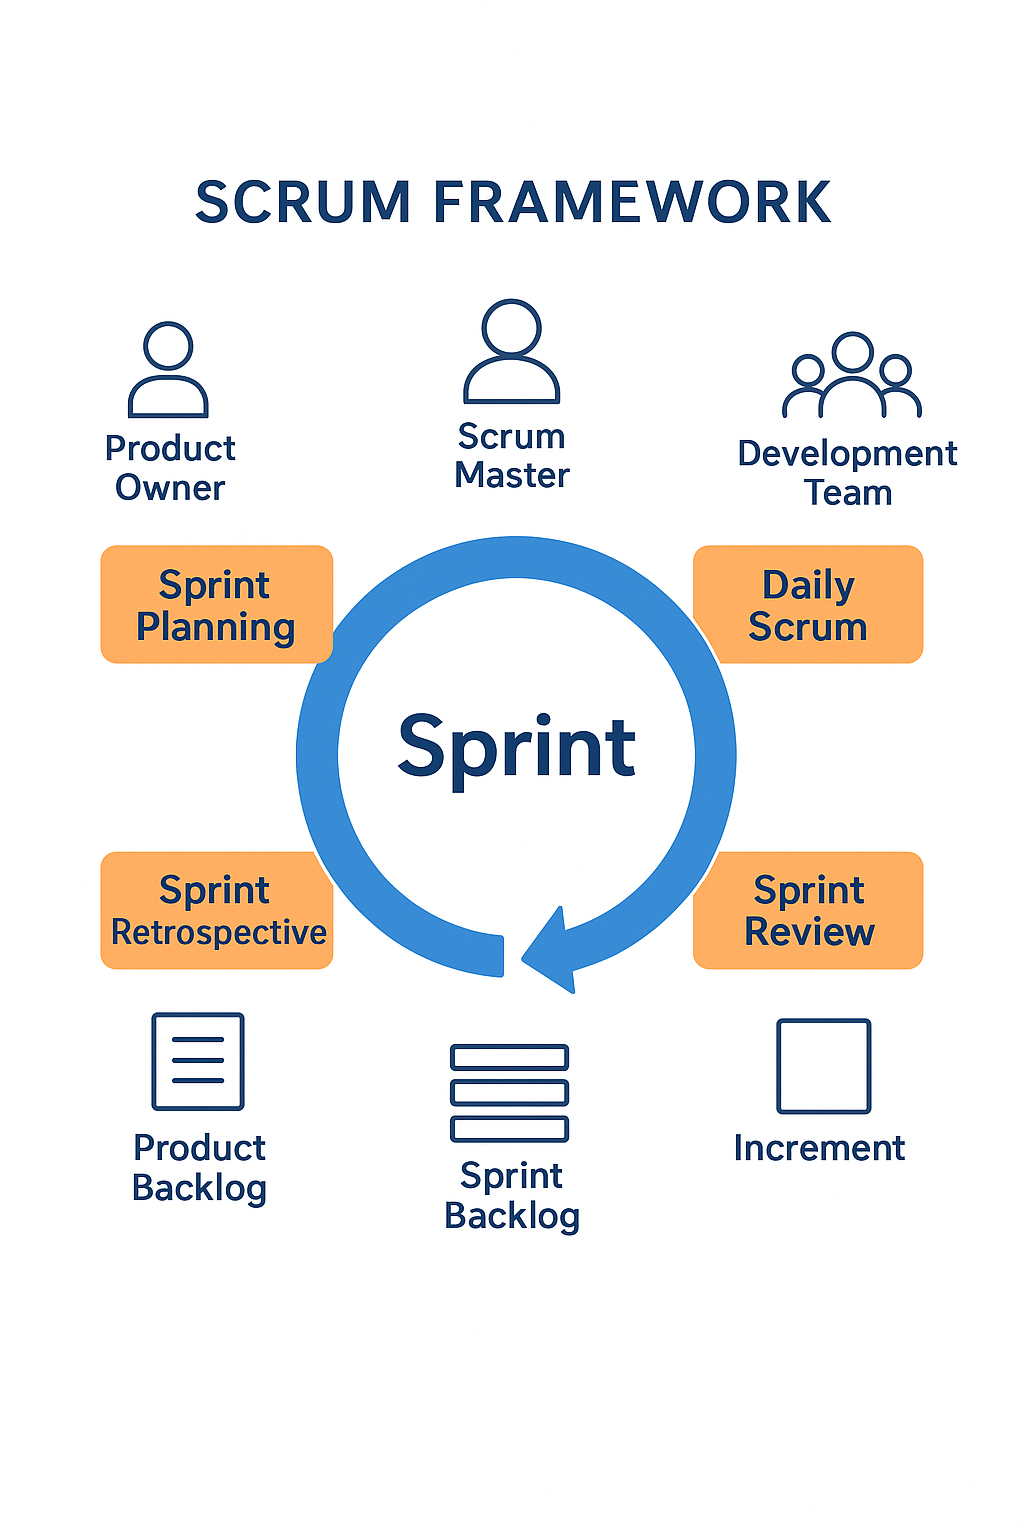
\includegraphics[width=0.9\textwidth]{chapters/chapter 1/figures/ScrumFramwork.png}
    \caption{The Scrum Framework}
    \label{fig:scrum}
\end{figure}

\section{Modeling Language}
The \textbf{Unified Modeling Language (UML)} was extensively used during the analysis and design phases to visualize, specify, and document the system's artifacts. The following diagrams were created to ensure a shared understanding of the system:
\begin{itemize}
    \item \textbf{Use Case Diagrams:} To capture functional requirements and interactions between actors and the system.
    \item \textbf{Class Diagrams:} To model the static structure of the system, showing the system's classes, attributes, methods, and relationships.
    \item \textbf{Sequence Diagrams:} To detail the dynamic interactions between objects for key processes and API calls.
    \item \textbf{Component/Architecture Diagrams:} To illustrate the high-level system components and their dependencies.
\end{itemize}
\begin{figure}[H]
    \centering
    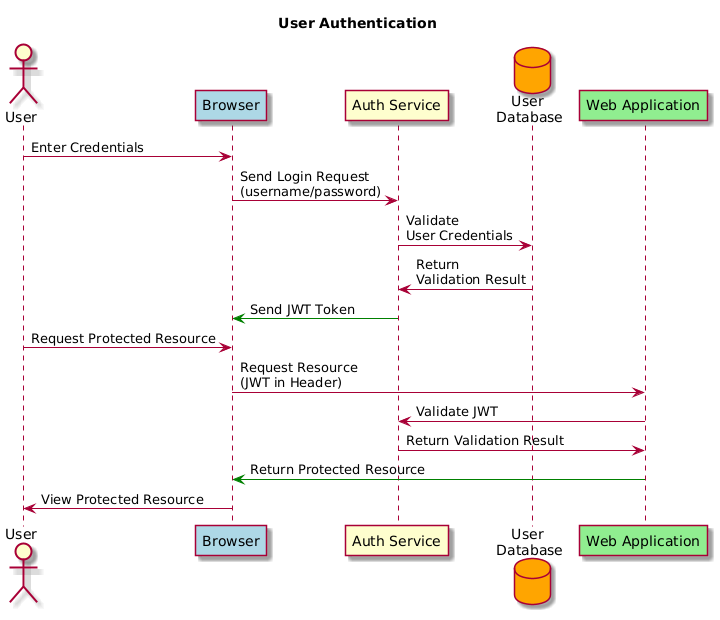
\includegraphics[width=0.7\textwidth]{chapters/chapter 1/figures/Sequence-Example2-1.png}
    \caption{Example UML Diagram (e.g., API Sequence Diagram)}
    \label{fig:uml}
\end{figure}

\section{Architecture}
The backend of the ERP system adheres to a layered \textbf{Model-View-Controller (MVC)} architecture. This promotes separation of concerns, making the codebase more organized, testable, and maintainable.
\begin{itemize}
    \item \textbf{Controller Layer:} Handles HTTP requests, invokes the necessary business logic from the Service layer, and returns appropriate HTTP responses.
    \item \textbf{Service Layer:} Contains the core business logic and rules, ensuring that controllers remain thin and logic is centralized and reusable.
    \item \textbf{Model Layer:} Utilizes Laravel's Eloquent ORM to represent business entities, manage data validation, and handle all data interactions with the database.
    \item \textbf{Database Layer:} Consists of the MySQL database, responsible for persistent and secure data storage.
\end{itemize}
This structured approach effectively separates the application's concerns, facilitating teamwork and enabling easier future enhancements.
\begin{figure}[H]
    \centering
    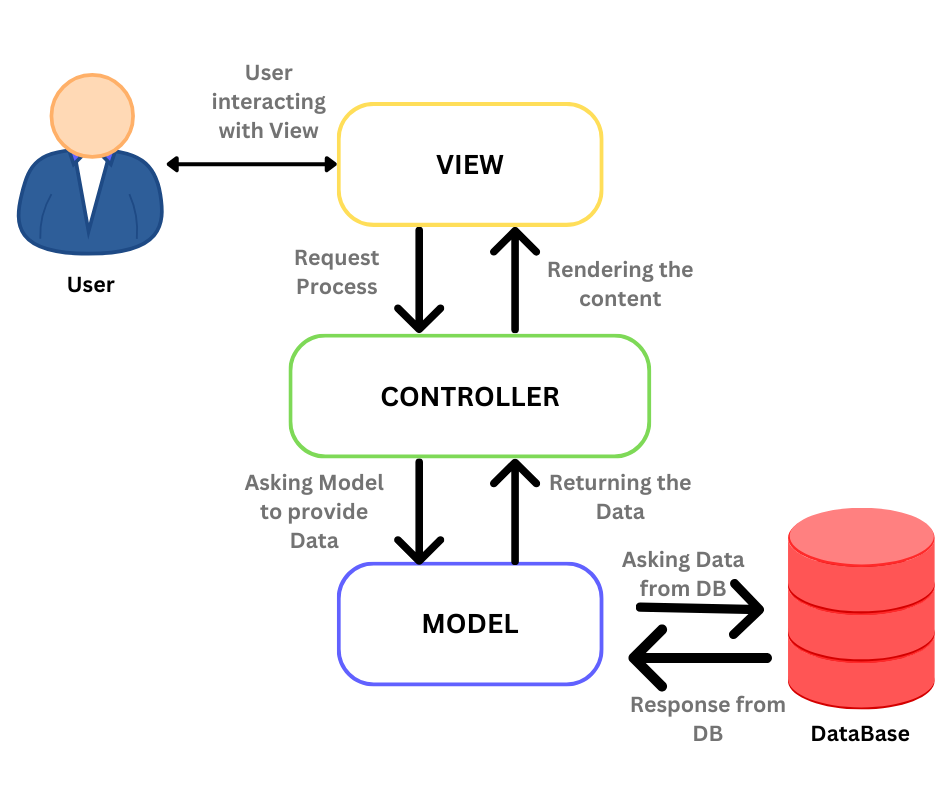
\includegraphics[width=0.8\textwidth]{chapters/chapter 1/figures/mvcArch.png}
    \caption{MVC Architecture of the Laravel Backend}
    \label{fig:mvc}
\end{figure}